\documentclass{article}
\usepackage{graphicx}
\usepackage{amsmath}
\usepackage{pgfplots}

\usepackage[a4paper, top=1cm, bottom=2cm, left=2cm, right=2cm, includehead, includefoot]{geometry}

\pgfplotsset{compat=1.18}

\begin{document}
\noindent
Physics 4A - Classical Mechanics \hfill Prof. Roger King

\noindent\rule{\textwidth}{0.4pt}

\begin{center}
    \textbf{\LARGE Chapter 2 - Motion Along a Straight Line} \\
    \vspace{12pt}
    \large Aaron W. Tarajos \\
    \textit{\today}
\end{center}

\noindent\rule{\textwidth}{0.4pt}

\section*{2.1 Position, Displacement, and Average Velocity}
\subsection*{key ideas}
\begin{itemize}
	\item The position $x$ of a particle on an $x$ axis locates the particle with respect to the origin
	\item The sign of the position indicates the direction the particle is located with respect to the origin
	\item Displacement $\Delta x$ is the change in position of the particle
		\[
			\Delta x = x_2-x_1
		\]
	\item Average velocity is the displacement of a particle over the time interval
		\[
			\nu_{avg} = \frac{\Delta x}{\Delta t} = \frac{x_2 - x_1}{t_2 - t_1}
		\]
	\item The sign of $\nu_{avg}$ indicates the direction of the motion with respect to the origin. Average velocity is not a function of distance traveled it is a function of initial and final position.
	\item On a graph of $x$ and $t$, average velocity is the slope of the line connecting two points on the graph.
	\item Average speed, $s_{avg}$ is the total distance travel over the time interval
		\[
			s_{avg} = \frac{\text{total distance}}{\Delta t}
		\]
\end{itemize}

\subsection*{2.1.1 Motion}
Kinematics is the classification and comparison of motions. Initially we restrict motion in a couple of ways to examine the most basic cases and get comfortable with the fundamental concepts of kinematics.
\begin{enumerate}
	\item We are only considering motion in a straight line--Newton didn't have a conception of curved space time so we don't need one either.
	\item The forces that cause motion are not considered, simply the motion itself and changes to motion.
	\item A moving object is either a point-like particle such as an electron or something rigid enough to behave like one. I.e. the whole body of the object moves at the same rate.
\end{enumerate}

\subsection*{2.1.2 Position and Displacement}
To locate an object means to find its position as a measure of length from the origin. In one dimension, movement to the right of the origin is positive and movement to the left of the origin is negative. The sign gives us a notion of direction and combined with the magnitude of the distance gives us our first vector quantity \textbf{displacement}.

Displacement, $\Delta x$, is not necessarily with respect to the origin it can be measured between any two points of an objects path of motion.
\[
	\Delta x = x_2-x_1
\]

\subsection*{2.1.3 Average Velocity and Average Speed}
We can think of change in position as a graph of plotted as a function of position $(x)$, and time $(t)$.

\begin{center}
\section*{Average Velocity Plot}
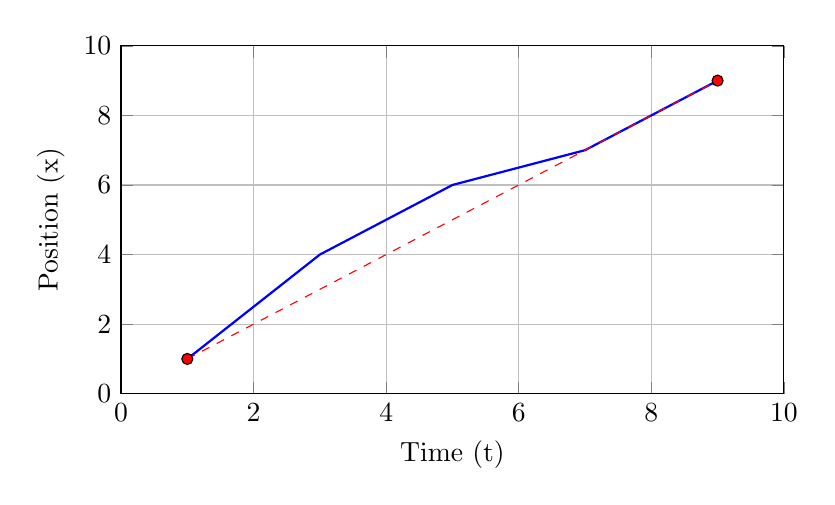
\begin{tikzpicture}
    \begin{axis}[
        xlabel={Time (t)},
        ylabel={Position (x)},
        grid=both,
        xmin=0, xmax=10,
        ymin=0, ymax=10,
        xtick={0,2,4,6,8,10},
        ytick={0,2,4,6,8,10},
        width=10cm,
        height=6cm
    ]
    % Plot the position-time graph
    \addplot[thick,blue] coordinates {(1,1) (3,4) (5,6) (7,7) (9,9)};

    % Highlight points for average velocity calculation
    \addplot[only marks,mark=*,mark options={fill=red}] coordinates {(1,1) (9,9)};

    % Draw a line representing the average velocity
    \addplot[dashed,red] coordinates {(1,1) (9,9)};

    \end{axis}
\end{tikzpicture}
\end{center}

\paragraph{Average Velocity:}
Average velocity, $\nu_{avg}$, is defined as the displacement (change in position) of an object over the time interval during which the displacement occurs:

\[
\nu_{avg} = \frac{\Delta x}{\Delta t} = \frac{x_2 - x_1}{t_2 - t_1}
\]
Here, $\Delta x$ is the displacement, and $\Delta t$ is the time interval. The sign of $\nu_{avg}$ indicates the direction of motion relative to the origin, making it a vector quantity. On a graph of position versus time, average velocity corresponds to the slope of the line connecting two points on the graph.

\paragraph{Average Speed:}
Average speed, $s_{avg}$, differs from average velocity as it considers the total distance traveled by the object rather than its displacement. It is defined as:

\[
s_{avg} = \frac{\text{total distance}}{\Delta t}
\]
Unlike average velocity, average speed is a scalar quantity and does not consider the direction of motion. It only accounts for how much ground an object has covered during the time interval.

\begin{itemize}
    \item \textbf{Average velocity} is a vector and depends on the net displacement, considering direction.
    \item \textbf{Average speed} is a scalar and only considers the total distance covered, irrespective of direction.
\end{itemize}

\section*{2.2 Instantaneous Velocity and Speed}\
\subsection*{key ideas}
\begin{itemize}
	\item The instantaneous velocity of a particle, $\nu$ is;
		\[
			\nu = \lim_{t \to 0} \frac{\Delta x}{\Delta t} = \frac{dx}{dt}
		\]
	\item If $\nu_{\text{avg}}$ is the slope of the line between two points then it is relatively intuitive that the instantaneous velocity is the derivative of the function $x(t)$.
	\item Speed is the magnitude of $\nu$, $|\nu|$.
\end{itemize}

There really isn't much to this section beyond the key ideas beyond the importance of the fact that speed is agnostic to direction and we cannot derive velocity from speed because it is not a vector quantity, it has incomplete information.

\section*{2.3 Acceleration}

\end{document}
